\documentclass[11pt]{article}
\usepackage[a4paper,margin=2cm]{geometry}
\usepackage[T1]{fontenc}
\usepackage{lmodern,microtype}
\usepackage{amsmath,booktabs}
\usepackage[authoryear,round]{natbib}
\usepackage[hidelinks]{hyperref}
\usepackage{url}
\usepackage{pgfplots}
\usepgfplotslibrary{groupplots}
\pgfplotsset{compat=1.18}
\usepackage{caption}
\captionsetup{font=small,labelfont=bf}
\setlength{\textfloatsep}{12pt plus 2pt minus 4pt}
\setlength{\intextsep}{6pt plus 2pt minus 2pt}
\bibpunct{(}{)}{;}{a}{,}{,}

% Colours: patient counts G = 5, 10, 20 (light to dark); mechanism arms.
\definecolor{gFive}{HTML}{FDAE61}
\definecolor{gTen}{HTML}{74ADD1}
\definecolor{gTwenty}{HTML}{313695}
\definecolor{cC}{HTML}{4575B4}

\title{\vspace{-1cm}\LARGE Patient Shortage in Histopathology Patch Classification\vspace{-0.5em}}
\author{Yannik Queisler}
\date{October 20, 2026}

\begin{document}
\maketitle

\section{Motivation}
Labelled histopathology data are scarce because expert annotation is expensive \citep{lu2021dataEfficient}. A labelling budget can cover many patches from few patients, or few patches from many patients. Patches from the same patient share morphology, staining and scanning conditions, so a large patch count from few patients may carry less evidence than its size suggests. Survey statistics captures this through the design effect: correlated observations within a cluster provide less information than the same number of independent observations \citep{kish1965survey}. It remains unclear whether this view explains the cost of patient shortage for a linear classifier on frozen foundation-model features. Whether that cost can be recovered without labelling more patients has not been measured in isolation.

\section{Setup}
Multinomial logistic regression is trained on frozen 2,560-dimensional Virchow2 patch features \citep{zimmermann2024virchow2} for two tasks: TCGA-UT, 30 cancer types from different organs \citep{komura2022universalEncoding}, and BRACS, 7 breast-lesion classes from normal tissue to invasive carcinoma \citep{brancati2022bracs}. Classes are balanced throughout, so only the composition of the training data varies. Each class receives exactly $G$ training patients with $m$ patches each, with $G\in\{5,10,20\}$ and $m\in\{8,16,32\}$. Cohorts are nested: the same patients appear at every depth, and each deeper patch set contains the shallower sets. The central comparison holds the budget at $Gm=160$ patches per class and shifts it from depth to breadth: five patients with 32 patches each, ten with 16, or twenty with 8. Validation and test patients are never resampled. The outcome is test patient-macro balanced accuracy (BA), which weights every class equally and, within each class, every patient equally. Intervals are paired 95\% Bayesian-bootstrap intervals over test patients \citep{rubin1981bayesian}. Differences of at least 1 percentage point (pp) count as material.

\section{Breadth beats depth at a fixed budget}
Spreading the same budget over more patients improves accuracy on both tasks (Figure~\ref{fig:grid}). At 160 patches per class, twenty patients with 8 patches each outperform five patients with 32 patches each by 3.71 pp [2.21, 5.35] on BRACS and by 9.52 pp [8.96, 10.07] on TCGA-UT. Accuracy rises steadily along this equal-budget line, with ten patients giving intermediate accuracy. The advantage holds in every split and for all 30 TCGA-UT cancer types.

\begin{figure}[!htb]
\centering
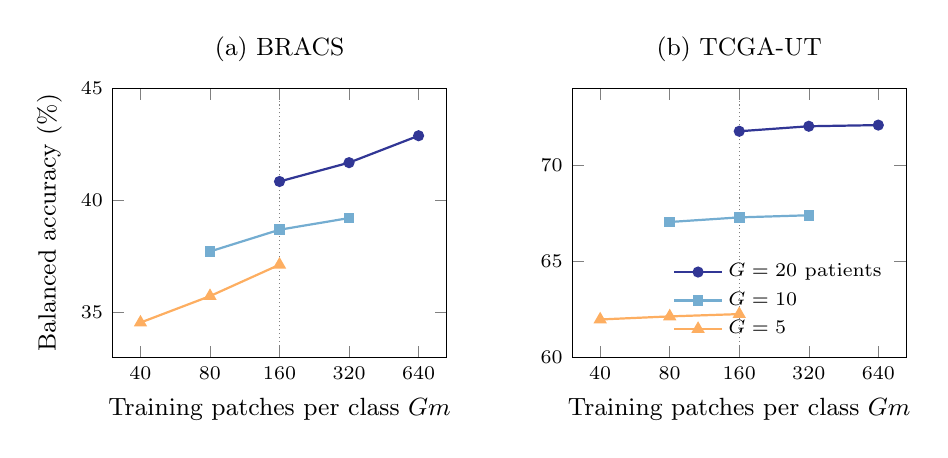
\begin{tikzpicture}
\begin{groupplot}[group style={group size=2 by 1,horizontal sep=1.6cm},
  width=0.48\textwidth,height=5cm,xmode=log,log basis x=2,
  xtick={40,80,160,320,640},xticklabels={40,80,160,320,640},
  xlabel={Training patches per class $Gm$},
  tick label style={font=\scriptsize},label style={font=\small},title style={font=\small},
  legend style={font=\scriptsize,at={(0.97,0.03)},anchor=south east,draw=none,fill=none},
  legend cell align=left]
\nextgroupplot[title={(a) BRACS},ylabel={Balanced accuracy (\%)},ymin=33,ymax=45]
\draw[densely dotted,gray] (axis cs:160,33) -- (axis cs:160,45);
\addplot[gTwenty,thick,mark=*,mark size=1.6pt] coordinates {(160,40.84)(320,41.68)(640,42.88)};
\addplot[gTen,thick,mark=square*,mark size=1.5pt] coordinates {(80,37.72)(160,38.69)(320,39.21)};
\addplot[gFive,thick,mark=triangle*,mark size=2pt] coordinates {(40,34.55)(80,35.73)(160,37.13)};
\nextgroupplot[title={(b) TCGA-UT},ymin=60,ymax=74]
\draw[densely dotted,gray] (axis cs:160,60) -- (axis cs:160,74);
\addplot[gTwenty,thick,mark=*,mark size=1.6pt] coordinates {(160,71.76)(320,72.02)(640,72.08)};
\addlegendentry{$G=20$ patients}
\addplot[gTen,thick,mark=square*,mark size=1.5pt] coordinates {(80,67.04)(160,67.28)(320,67.39)};
\addlegendentry{$G=10$}
\addplot[gFive,thick,mark=triangle*,mark size=2pt] coordinates {(40,61.97)(80,62.13)(160,62.25)};
\addlegendentry{$G=5$}
\end{groupplot}
\end{tikzpicture}
\caption{Adding patients raises accuracy far more than adding patches from the same patients. Each line keeps the patients fixed and increases depth from $m=8$ to 32 patches per patient. The dotted line marks the equal budget of 160 patches per class, where the three cohorts differ only in how the budget is spread over patients.}
\label{fig:grid}
\end{figure}

The two tasks differ in the value of depth. Quadrupling the patches per patient in a twenty-patient cohort adds 2.04 pp [1.13, 2.93] on BRACS but only 0.32 pp [0.24, 0.41] on TCGA-UT, where accuracy is practically saturated beyond 8 patches per patient. Dataset construction explains the difference. TCGA-UT patches are rotated and rescaled crops of a few uniform tumour regions per slide \citep{komura2022universalEncoding}, whereas BRACS patches tile each annotated region without overlap \citep{brancati2022bracs}. Accordingly, the intraclass correlation of patch features within a patient averages 0.457 on TCGA-UT and 0.130 on BRACS. Thus, 32 patches from one TCGA-UT patient count as roughly two independent observations, compared with six on BRACS.

This redundancy explains the BRACS grid but not the TCGA-UT grid. On BRACS, effective support---the patch count divided by the design effect \citep{kish1965survey}---places all nine allocations close to one line. Patient count adds no explanatory value once effective support is known. On TCGA-UT, each doubling of patients still adds 2.98 pp [2.47, 3.46] beyond the gain in effective observations, and 2.62 pp when correlation is measured across all feature directions. Neither a multilayer perceptron nor a nearest-neighbour classifier recovers the deficit. Weighting every patient equally in the loss changes accuracy by at most 1.4 pp, leaving the benefit of more patients intact.

The benefit also extends to predicted probabilities. After temperature scaling, the broad allocation still lowers the negative log-likelihood by 0.12 nats on BRACS and 0.39 nats on TCGA-UT, whereas its advantage in calibration error almost disappears. Temperature scaling therefore corrects the confidence level of a model trained on few patients, but not its misplaced probability mass.

\section{Cohort composition}
At a fixed patient count, the choice of patients matters. On TCGA-UT, a cohort of twenty patients from one neighbourhood in feature space yields accuracy 8.30 pp [7.66, 8.95] below that of twenty random patients, nearly the full cost of having five instead of twenty patients. Conversely, selecting five patients to cover the other training patients as evenly as possible raises accuracy by 5.52 pp [4.83, 6.23] over five random patients. Selection uses only training-pool features, without access to validation or test patients. It thus recovers 58\% of the gap to twenty random patients without labelling additional patients. A model fitted to cohorts with independently varied coverage and similarity attributes roughly half of the predicted selection gain to low similarity among selected patients and half to their coverage of validation patients. This attribution extrapolates beyond the similarity range of the designed cohorts. Coverage cannot replace patient count, however. In the designed cohorts, ten patients still yield higher accuracy even when they cover validation patients less well than five random patients do.

\section{Class-centre error carries the patient benefit}
A linear classifier depends first on where each class lies in feature space. Write a patch feature of class $c$ as $\mathbf x=\boldsymbol\mu_c+\mathbf u_i+\mathbf e$, where $\boldsymbol\mu_c$ is the class centre, $\mathbf u_i$ is the offset of patient $i$ with covariance $\boldsymbol\Sigma_B$, and $\mathbf e$ is the within-patient residual with covariance $\boldsymbol\Sigma_W$. A cohort of $G$ patients with $m$ patches each then estimates the centre with error covariance
\begin{equation}
  \operatorname{Cov}(\hat{\boldsymbol\mu}_c-\boldsymbol\mu_c)=\frac{\boldsymbol\Sigma_B}{G}+\frac{\boldsymbol\Sigma_W}{Gm}.
  \label{eq:centre}
\end{equation}
At a fixed budget $Gm$, the second term is constant, so only additional patients reduce centre error. When patches from the same patient are highly similar, as on TCGA-UT, the first term dominates and depth adds almost nothing.

Experiments that change only the class centres of the training cohort test this account (Figure~\ref{fig:centre}). Shifting each class mean to the mean of all eligible training patients of that class leaves every patch's offset from its class mean unchanged. With correct centres, a five-patient cohort outperforms a real twenty-patient cohort by 1.25 pp [0.73, 1.73] on TCGA-UT and 3.66 pp [1.83, 5.54] on BRACS. Correct centres remove 74\% [70, 78] of the five-to-twenty-patient gap on TCGA-UT and 82\% [59, 102] on BRACS, with the same share for each doubling. Conversely, random centre error of the size that Equation~\eqref{eq:centre} predicts for $G$ patients reproduces 88\% [79, 97] and 99\% [53, 182] of the real gap, respectively. Two controls locate the harmful error. Shifting the class centres of a five-patient cohort to those of another five-patient cohort gains 0.21 pp [$-0.62$, 1.17]. The gain thus comes from accurate centres rather than shifting alone. Correcting only the error shared by all classes, such as a common stain or scanner offset, gains 0.14 pp. The error that costs accuracy is therefore specific to each class.

\begin{figure}[!htb]
\centering
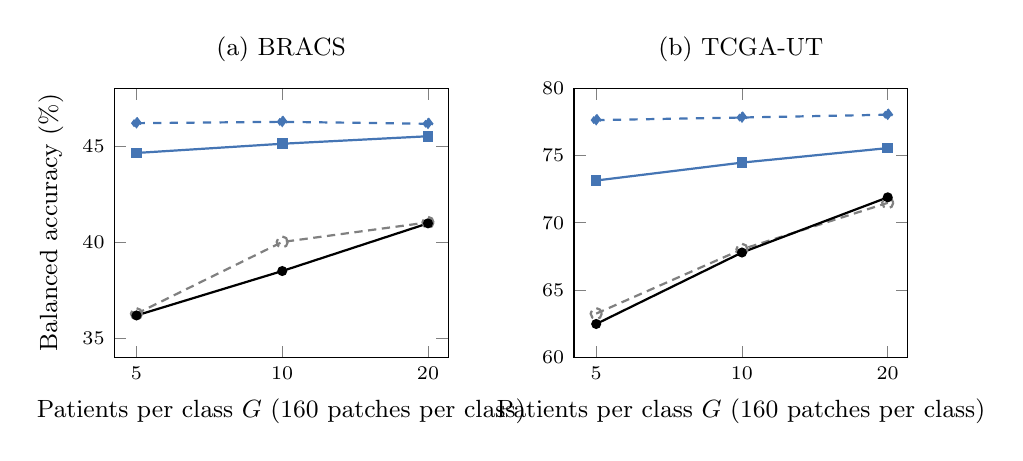
\begin{tikzpicture}
\begin{groupplot}[group style={group size=2 by 1,horizontal sep=1.6cm},
  width=0.48\textwidth,height=5cm,xmode=log,log basis x=2,
  xtick={5,10,20},xticklabels={5,10,20},xmin=4.5,xmax=22,
  xlabel={Patients per class $G$ (160 patches per class)},
  tick label style={font=\scriptsize},label style={font=\small},title style={font=\small},
  legend style={font=\scriptsize,draw=none,legend columns=4,column sep=6pt},
  legend to name=centreleg,legend cell align=left]
\nextgroupplot[title={(a) BRACS},ylabel={Balanced accuracy (\%)},ymin=34,ymax=48]
\addplot[cC,thick,dashed,mark=diamond*,mark size=2pt] coordinates {(5,46.18)(10,46.25)(20,46.15)};
\addplot[cC,thick,mark=square*,mark size=1.5pt] coordinates {(5,44.63)(10,45.11)(20,45.50)};
\addplot[gray,thick,densely dashed,mark=o,mark size=2pt] coordinates {(5,36.27)(10,40.00)(20,41.02)};
\addplot[black,thick,mark=*,mark size=1.4pt] coordinates {(5,36.18)(10,38.49)(20,40.97)};
\nextgroupplot[title={(b) TCGA-UT},ymin=60,ymax=80]
\addplot[cC,thick,dashed,mark=diamond*,mark size=2pt] coordinates {(5,77.63)(10,77.82)(20,78.03)};
\addlegendentry{correct centres, whitened}
\addplot[cC,thick,mark=square*,mark size=1.5pt] coordinates {(5,73.14)(10,74.47)(20,75.55)};
\addlegendentry{correct centres}
\addplot[gray,thick,densely dashed,mark=o,mark size=2pt] coordinates {(5,63.25)(10,68.03)(20,71.48)};
\addlegendentry{simulated centre error}
\addplot[black,thick,mark=*,mark size=1.4pt] coordinates {(5,62.48)(10,67.79)(20,71.89)};
\addlegendentry{real cohort}
\end{groupplot}
\end{tikzpicture}\\[2pt]
\ref{centreleg}
\caption{Correct class centres make patient count nearly irrelevant, and simulated centre error of the size expected for $G$ patients restores the real accuracy curve. Correct centres are the means of all eligible training patients of a class; whitening additionally shrinks the directions in which training patients differ. On these independent draws, the real five-to-twenty-patient gap is 4.80 percentage points on BRACS and 9.41 percentage points on TCGA-UT.}
\label{fig:centre}
\end{figure}

A second, smaller channel lies in the directions along which patients differ. Whitening the features along the between-patient directions of the training population removes 25\% [21, 29] of the TCGA-UT gap on its own. Its effect adds to that of correct centres, and together they remove 96\% of the gap; the remaining patient benefit is 0.40 pp [0.23, 0.57]. On BRACS, the two remedies together close the gap completely, but their effects overlap. Whitening gains 3.33 pp on real five-patient cohorts and only 1.55 pp once their centres are correct, so it works there largely by reducing centre error. Across both tasks, the value of an additional patient lies mainly in where it places the class centre. This account also unifies the redundancy results: effective support counts independent observations, but only patients reduce the between-patient term of Equation~\eqref{eq:centre}.

\section{Cohort-only remedies recover little}
Correct centres improve accuracy by 10.66 pp on TCGA-UT and 8.45 pp on BRACS at five patients, but require all training patients. A practical remedy can use only the drawn cohort. Four such remedies target the two channels (Table~\ref{tab:remedies}). James--Stein shrinkage pulls each class centre towards the cohort's grand mean \citep{james1961}. Directional shrinkage does the same along the cohort's between-patient eigendirections, with strong shrinkage where centre differences are no larger than patient noise. Cohort whitening uses the cohort's between-patient directions instead of the population's. Centre-uncertainty training leaves the centres unchanged and trains the classifier under Gaussian centre perturbations with the cohort's own patient covariance. It uses the implicit semantic data augmentation bound on cross-entropy \citep{wang2019isda}.

\begin{table}[!htb]
\centering\small
\setlength{\tabcolsep}{5pt}
\begin{tabular}{@{}llrr@{}}
\toprule
Method & Information used & TCGA-UT & BRACS \\
\midrule
James--Stein centre shrinkage & cohort & 0.14 [$-0.01$, 0.29] & 0.98 [0.23, 1.84] \\
Directional centre shrinkage & cohort & 1.29 [0.99, 1.57] & 0.36 [$-0.31$, 1.11] \\
Cohort whitening & cohort & 2.26 [1.97, 2.54] & 0.32 [$-0.36$, 1.22] \\
Centre-uncertainty training & cohort & 2.34 [2.03, 2.63] & 0.25 [$-0.37$, 0.97] \\
\addlinespace
Coverage-maximizing selection & unlabelled pool features & 5.52 [4.83, 6.23] & -- \\
\addlinespace
Population whitening (reference) & all training patients & 4.92 [4.47, 5.32] & 3.33 [1.65, 5.27] \\
Correct centres (reference) & all training patients & 10.66 [9.78, 11.47] & 8.45 [6.31, 10.84] \\
Twenty real patients (reference) & 15 more patients & 9.41 [8.71, 10.12] & 4.80 [2.88, 6.75] \\
\bottomrule
\end{tabular}
\caption{Remedies that use only the five drawn patients recover up to 22\% of the centre-error headroom on TCGA-UT. On BRACS, James--Stein shrinkage has an interval entirely above zero, but no cohort-only remedy establishes a gain above the practical threshold of 1 percentage point. Entries are balanced accuracy gains over the real five-patient cohort in percentage points with 95\% intervals; remedy strengths are tuned on validation patients. Selection is compared with the random cohort sharing its first patient and was tested on TCGA-UT only. Reference rows use information a practitioner does not have.}
\label{tab:remedies}
\end{table}

Centre shrinkage fails because the cohort cannot reveal where its centres are wrong. James--Stein shrinkage removes 21\% of the squared centre error on TCGA-UT, but only along the line from the grand mean to the class centre. This line is the class's own discriminative axis, so the class signal shrinks together with the error. Directional shrinkage gains 1.29 pp on TCGA-UT, yet barely reduces centre error; it acts like a weak form of whitening. Cohort whitening and centre-uncertainty training both gain about 2.3 pp on TCGA-UT at five patients, recovering about 22\% of the headroom. Because its gain persists at twenty patients, centre-uncertainty training narrows the five-to-twenty-patient gap by only 1.02 pp [0.71, 1.34]. On BRACS, only James--Stein shrinkage has an interval entirely above zero, and no cohort-only remedy reaches the 1-pp threshold with confidence.

The ceiling of the whitening remedies lies in the directions the cohort can observe, not in how it weights them. Five TCGA-UT patients per class span 70\% of the population's between-patient variance. Correcting the cohort's noisy eigenvalues gains 0.08 pp, and adding within-patient patch directions from the same patients gains 0.45 pp. These directions reach the missing subspace but are oriented incorrectly within it. Using the population's own eigenbasis in the same subspace would close 80\% of the remaining gap to population whitening on TCGA-UT and 77\% on BRACS. A small cohort carries no patient-level information that could identify these directions. Recovering the patient benefit therefore requires information from outside the labelled cohort.

\begin{samepage}
\section{Implications for annotation and mitigation}
\begin{itemize}\setlength{\itemsep}{1pt}
\item Spread a labelling budget over many patients with few patches each. On datasets built from repeated crops of curated regions, such as TCGA-UT, depth beyond 8 patches per patient adds less than 0.5 pp.
\item Choose which patients to label. Coverage-maximizing selection from unlabelled features recovers 58\% of the patient gap, and a cohort of similar patients costs nearly as much as losing three quarters of the patients.
\item Changing the classifier, weighting patients equally, or applying temperature scaling does not substitute for patient breadth; its likelihood advantage survives temperature scaling.
\item Target the class centre. At five patients, remedies that rely on the labelled cohort alone recover up to 22\% of the centre-error headroom on TCGA-UT; promising sources of outside information are unlabelled slides of the same classes, related classes, and other cohorts.
\end{itemize}
\end{samepage}

\appendix
\raggedright
\section{Guide to the supporting experiments}
The numbered folders below are under \path{experiments/02_patient_shortage/}. Each folder's \path{report/} directory contains a PDF and its LaTeX source, covering the protocol, full tables and uncertainty estimates.

\noindent\textbf{Headline results.}
\begin{itemize}\setlength{\itemsep}{2pt}
\item \textbf{Breadth versus depth:} Report 05, in \path{00_damage/05_effective_support/report/}, gives the nine-cell grid, the equal-budget contrast, effective-support regressions, probability quality and class-level recalls on both datasets.
\item \textbf{Classifier and loss weighting:} Reports 03 and 04, in \path{01_cause/03_classifier_limitation/report/} and \path{01_cause/04_patient_influence/report/}, show that neither changing the classifier nor weighting patients equally recovers the deficit.
\item \textbf{Cohort composition and selection:} Reports 10, 12 and 14, in \path{01_cause/10_cohort_composition/report/}, \path{01_cause/12_shortage_selection/report/} and \path{01_cause/14_shortage_decomposition/report/}, measure clustered and dispersed cohorts, coverage-maximizing selection, and the split of the gap into coverage, similarity and patient count.
\item \textbf{Centre-error mechanism:} Reports 16, 17 and 18, in \path{01_cause/16_centre_error/report/}, \path{01_cause/17_patient_directions/report/} and \path{01_cause/18_bracs_mechanism/report/}, give the centre, simulated-error and whitening arms on TCGA-UT and BRACS.
\item \textbf{Cohort-only remedies:} Reports 19--21, in \path{02_mitigation/19_centre_shrinkage/report/}, \path{02_mitigation/20_directional_shrinkage/report/} and \path{02_mitigation/21_centre_uncertainty/report/}, evaluate the four remedies of Table~\ref{tab:remedies}.
\end{itemize}

\noindent\textbf{Further reading.} Reports 06 and 07 test full-feature redundancy and tissue-source-site coverage as explanations of the TCGA-UT residual. Reports 08, 09, 11, 13 and 15 document coverage designs that stopped at their manipulation or precision checks, or remained inconclusive. Reports 22--24 explain why cohort whitening stops at about 2.3 pp: eigenvalue correction, within-patient directions and oracle weights on those directions.

\clearpage
\bibliographystyle{abbrvnat}
\bibliography{references}
\end{document}
